\subsection{Overordnet teknisk koncept}
Vores app som skal håndtere subscription fatigue, skal overholde følgende tekniske krav:
\begin{itemize}
    \item \textbf{Programmeres via React Native} (expo)\\
    Appen bliver udviklet via teknikker som benyttes i den virkelige softwareudviklingsindustri, og bygger på React som er et \textit{Framework}\footnote{Et framework understøtter programmeringen af diverse applikationer, her muliggør det Javascript at blive lavet om til eksekverbar filer som kan køre på diverse mobiltelefoner til programmeringssporget JavaScript} til JavaScript
    \item \textbf{Trække data fra en given brugeres telefon og fortage statestik over det.}\\
    Udataen skal helt konkret hentes via et element i expo-biblioteket(getUsage), som brugres mobiltelefonens indbyggede statestiksystem til at se hvor lang tid en given app har været i brug. 
    \item 
\end{itemize}


\subsection{Overordnet om produktudvikling}
Den konkrete udvikling af produktet påbegyndes herfra.

Når der arbejdes med at skabe et digitalt produkt, arbejder man som regl altid med en iterativ udviklingsprocess. Det betyder at man 
\begin{figure}[H]
    \centering
    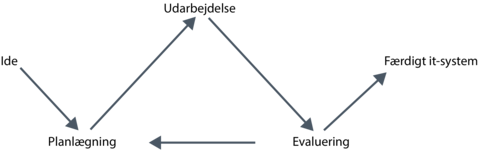
\includegraphics[width=0.5\textwidth]{assets/trinvis_forbedring.png}
    \caption{Iterativ udviklingsproces}
\end{figure}

Vigtigheden af løbende test og evaluering...


\subsection{Test}
Specifikt om test og testmetoder...

\subsubsection{Usibility Test}
\subsubsection{A/B Testing}
